%%%%%%%%%%%%%%%%%%%%%%%%%%%%%%%%
% INSTRUCTION SET ARCHITECTURE (ISA)

\lecture{Conjunto de instruções: a linguagem do computador}{isa}

\lecturetitle{\insertlecture}{\course}

\frame{\maketitle}

\section{Introdução}

%\framevonneumannarch{}

%\framefigtanenbaum{}

\lecture{Operações do hardware do computador}{isa:ops}

\begin{frame}{\insertlecture}
 \begin{block}{Operações básicas}
  \begin{itemize}
  \item Aritmética
    \begin{itemize}
    \item Adição,
    \item Subtração,
    \item Multiplicação,...
    \end{itemize}
  \item Manipulação de dados - modelo {\em load$\slash$store}
    \begin{itemize}
    \item Carga ({\em load});
    \item Armazenamento ({\em store}). 
    \end{itemize}
  \end{itemize}
\end{block}
\end{frame}

\begin{frame}{Linguagem de montagem ({\em assembly})}
  
  \begin{block}{Arquitetura MIPS? Por quê?}
    \begin{itemize}
    \item Conjunto reduzido de instruções favorecendo simplicidade;
    \item Maior quantidade de registradores quando comparada com
      outras arquiteturas;
    \item Utilização de arquiteturas semelhantes em grande escala
      (SPARC, ARM, PowerPC,...);
    \item Simuladores disponíveis para aprendizado.
    \end{itemize}
  \end{block}
\end{frame}

\begin{frame}{Sequência de geração de código binário}
  

%%% Local Variables: 
%%% mode: latex
%%% TeX-master: t
%%% End: 

\usetikzlibrary{shapes}
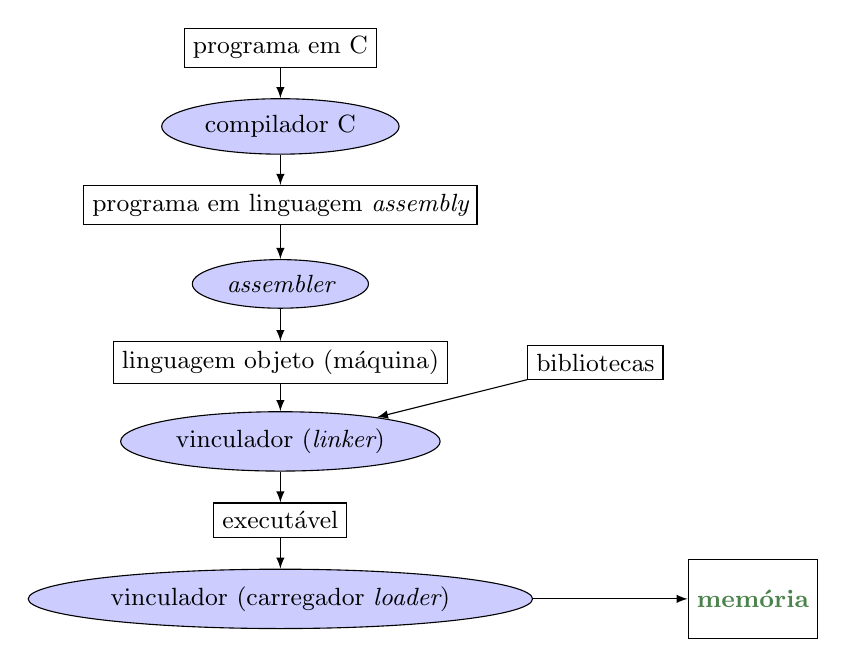
\begin{tikzpicture}[]
\small
  \node[rectangle,draw] (cprog) {programa em C};
  \node[fill=blue!20,ellipse,draw] (ccomp) [below of=cprog] {compilador C};
    \node[rectangle,draw] (sprog) [below of=ccomp] {programa em linguagem {\em
        assembly}};
    \node[fill=blue!20,ellipse,draw] (scomp) [below of=sprog] {{\em assembler}};
    \node[rectangle,draw] (mach) [below of=scomp] {linguagem objeto
      (máquina)};
    \node[rectangle,draw] (lib) [right of=mach,xshift=30mm] {bibliotecas};
    \node[fill=blue!20,ellipse,draw] (linker) [below of=mach] {vinculador ({\em linker})};
    \node[rectangle,draw] (exe) [below of=linker] {executável};
    \node[fill=blue!20,ellipse,draw] (loader) [below of=exe] {vinculador (carregador {\em
        loader})};
    \node[rectangle,minimum height=1cm,draw] (mem) [right of=loader,xshift=50mm] {\bf \color{green!30!black!70!}memória};
    
    \draw[->,>=latex] (cprog) -> (ccomp);
    \draw[->,>=latex] (ccomp) -> (sprog);
    \draw[->,>=latex] (sprog) -> (scomp);
    \draw[->,>=latex] (scomp) -> (mach);
    \draw[->,>=latex] (mach) -> (linker);
    \draw[->,>=latex] (lib) -> (linker);
    \draw[->,>=latex] (linker) -> (exe);
    \draw[->,>=latex]  (exe) -> (loader);
    \draw[->,>=latex] (loader) -> (mem);

\end{tikzpicture}

\end{frame}

\begin{frame}{Alocação de memória feita pelo carregador ({\em linker})}
  
\begin{center}

%%% Local Variables: 
%%% mode: latex
%%% TeX-master: t
%%% End: 

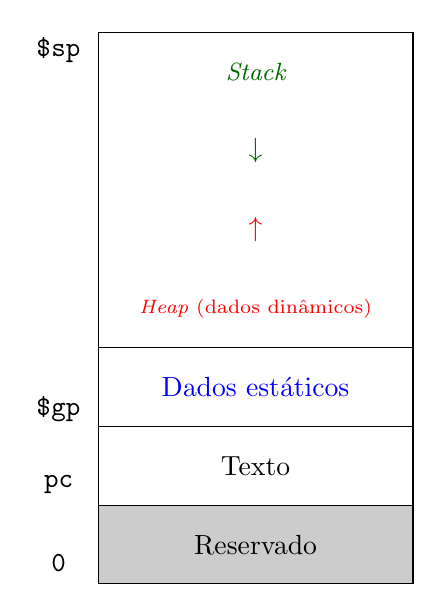
\begin{tikzpicture}
  \node[rectangle,draw,minimum width=4cm,minimum
  height=1cm,fill=gray!40]  (reserved) {Reservado};
  \node[rectangle,draw,minimum width=4cm,minimum
  height=1cm] (text) [above of=reserved] {Texto};
  \node[rectangle,draw,minimum width=4cm,minimum
  height=1cm] (static) [above of=text] {\color{blue}Dados estáticos};
  \node (heap) [above of=static] {\scriptsize \color{red}{\em Heap} (dados
    dinâmicos)};
  \node (up) [above of=heap] {\color{red}$\uparrow$};
  \node (down) [above of=up] {\color{green!40!black}$\downarrow$};
  \node (stack) [above of=down] {\small {\color{green!40!black}\em Stack}};
  \node[rectangle,draw,minimum width=4cm,minimum height=6cm,yshift=5mm] (rect) [above of=static] {};

  \node [left of=reserved,xshift=-15mm,anchor=north] {\tt 0};
  \node [left of=text,xshift=-15mm,anchor=north] {\tt pc};
  \node [left of=static,xshift=-15mm,anchor=north] {\tt \$gp};
  \node [left of=stack,xshift=-15mm,anchor=south] {\tt \$sp};

\end{tikzpicture}
\end{center}

\end{frame}

\lecture{Operações aritméticas}{isa:arith}

\section{\insertlecture}

\begin{frame}[fragile]{Compilando C para MIPS}
$\Rightarrow$ compilador\\

a $\leftarrow$ \$s0, {\color{blue} b $\leftarrow$ \$s1}, 
{\color{red}c $\leftarrow$ \$s2}, { d
  $\leftarrow$ \$s3},
{ \color{green!50!black!90!}  e $\leftarrow$ \$s4}\\

\bigskip
  \begin{minipage}[h]{0.275\linewidth}
    \begin{tabbing}
      a \= $=$ \= {\color{blue}b} \= $+$ \= {\color{red}c}; $\Rightarrow$\\
      d \> $=$ \> a \> $-$ \> {\color{green!50!black!90!}e}; $\Rightarrow$\\
    \end{tabbing}
  \end{minipage}
  \only<2->{
  \begin{minipage}[h]{0.7\linewidth}
    \small
    \begin{tt}
      {\bf add} \$s0,{\color{blue}\$s1},{\color{red}\$s2} {\color{gray}\footnotesize \# registro \$s0 recebe b + c}\\
      {\bf sub} \$s3,\$s0,{\color{green!50!black!90!}\$s4} {\color{gray}\footnotesize \# registro \$s3 recebe a - e}\\
    \end{tt}
  \end{minipage}
}

\bigskip

\small
\only<3->{
Como um compilador poderia converter a seguinte atribuição em C?\\
\begin{tt}
  \begin{tabbing}
expressão:    \=f  = (\=g + \=h) - (\=i + \=j);\\
    \>| \>| \>| \>| \>|\\
registros:    \>\$s0 \>\$s1 \>\$s2 \>\$s3 \>\$s4
  \end{tabbing}
\end{tt}
}

\only<4->{
\begin{tt}
  {\bf add} \$t0,\$s1,\$s2 {\color{gray}\footnotesize \# registro \$t0 recebe g + h}\\
  {\bf add} \$t1,\$s3,\$s4 {\color{gray}\footnotesize \# registro \$t1
    recebe i + j}\\
  {\bf sub} \$s0,\$t0,\$t1 {\color{gray}\footnotesize \# f recebe \$t0 -
    \$t1 $\equiv$ (g + h) - (i + j)}\\
\end{tt}
}
\end{frame}


\begin{frame}[fragile]{Operações aritméticas com constantes}
$\Rightarrow$ compilador\\

a $\leftarrow$ \$s0, {\color{blue} b $\leftarrow$ \$s1}, 
c $\leftarrow$ \$s2\\

\bigskip
  \begin{minipage}[h]{0.275\linewidth}
    \begin{tabbing}
      a \= $=$ \= {\color{blue}b} \= $+$ \= {\color{red}20}; $\Rightarrow$\\
      c \> $=$ \> a \> $-$ \> {\color{green!50!black!90!}8}; $\Rightarrow$\\
    \end{tabbing}
  \end{minipage}
  \only<2->{
  \begin{minipage}[h]{0.7\linewidth}
    \small
    \begin{tt}
      {\bf addi} \$s0,{\color{blue}\$s1},{\color{red}20} {\color{gray}\footnotesize \# registro \$s0 recebe b + 20}\\
      {\bf subi} \$s2,\$s0,{\color{green!50!black!90!}8} {\color{gray}\footnotesize \# registro \$s3 recebe a - 8}\\
    \end{tt}
  \end{minipage}
}

\bigskip
-- Inicialização\\
\only<3->{
  \begin{minipage}[h]{0.275\linewidth}
    \begin{tabbing}
      a \= $=$ \= {\color{blue}0}; $\Rightarrow$\\
    \end{tabbing}
  \end{minipage}
}
\only<4->{
  \begin{minipage}[h]{0.7\linewidth}
    \small
    \begin{tt}
      {\bf move} \$s0,\$zero {\color{gray}\footnotesize \# \$s0
        recebe o valor zero}\\
    \end{tt}
  \end{minipage}
}
\end{frame}

\section{Exercícios I}

\begin{frame}{Exercícios I}
  \begin{itemize}

  \item Operações aritméticas
    \begin{enumerate}
    \item $f = g + (j + 2)$
    \item $f=f+g+h+i+j+2$
    \item $f=g- (f - 5)$
    \end{enumerate}
    \bigskip
  \end{itemize}
  
\end{frame}


\lecture{MIPS: Operações em Memória}{isa:mem}

\lecturetitle{\insertlecture}{\course}

\frame{\maketitle}

\section{\insertlecture}

\begin{frame}{Operações de memória - {\bf Carga}--MIPS}{{\em\bf Load}--MIPS}
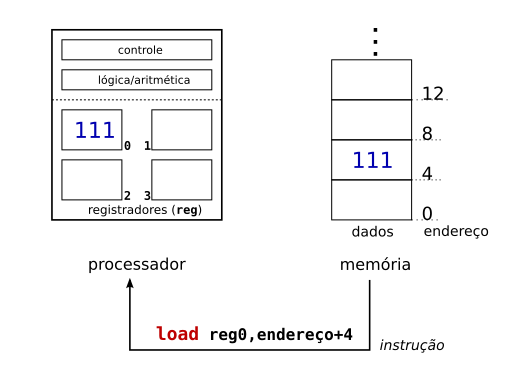
\includegraphics[scale=0.7]{instr_mem_load.png}
\end{frame}

\begin{frame}{Operações de memória - {\bf Carga}--MIPS}{{\em\bf Load}--MIPS}
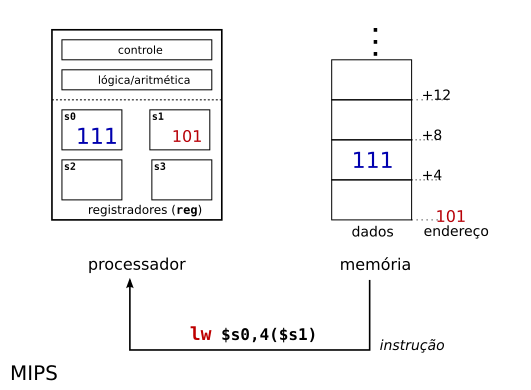
\includegraphics[scale=0.7]{instr_mem_load_mips.png}
\end{frame}

\begin{frame}{Operações de memória - {\bf Armazenamento}}{{\em\bf Store}}
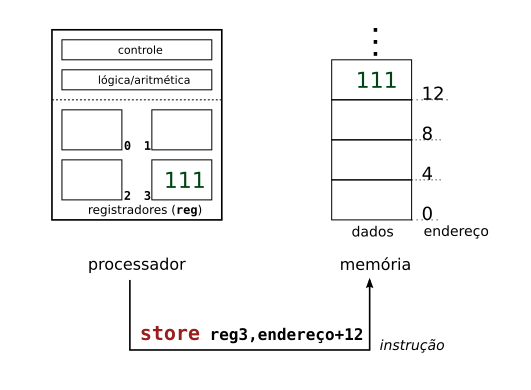
\includegraphics[scale=0.7]{instr_mem_store.png}
\end{frame}

\begin{frame}{Operações de memória - {\bf Armazenamento}--MIPS}{{\em\bf Store}--MIPS}
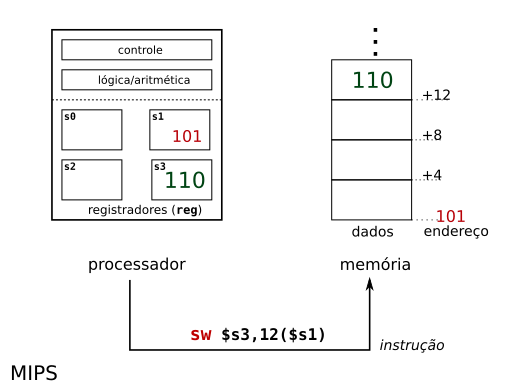
\includegraphics[scale=0.7]{instr_mem_store_mips.png}
\end{frame}


\section{Exercícios II}

\def\mem{{\footnotesize\color{gray}\# (M)}}
\begin{frame}{Exercícios II}
  \large

\begin{itemize}
\item Memória
  \begin{enumerate}
  \item $f = g + B[4]$ \mem
  \item $ f = g - A[B[4]]$ \mem
  \end{enumerate}

  \bigskip
  {\footnotesize (M) -- codificar instruções de transferência entre a
    memória e o processador.}
  
\end{itemize}

\end{frame}

\lecture{Formato das instruções MIPS}{isa:mips:format}

\section{\insertlecture}

\begin{frame}{\insertlecture}{Formato R}
  \def\mywidth{1.75cm}
  \def\myheight{0.75cm}

\begin{block}{Formato R (registro)}
  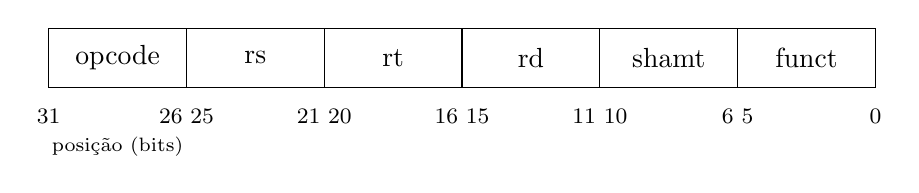
\begin{tikzpicture}
    \foreach \x/\field/\pos in {0/opcode/31,1/rs/{26 25},2/rt/{21
        20},3/rd/{16 15},4/shamt/{11 10},5/funct/{6 5}} {
      \draw (\x*\mywidth,0) rectangle (\x*\mywidth+\mywidth,\myheight);
      \node at (\x*\mywidth+\mywidth/2, \myheight/2) {\field};
      \node at (\x*\mywidth, -\myheight/2) {\footnotesize\pos};
    }
    \node at (6*\mywidth, -\myheight/2) {\footnotesize 0};
    \node at (\mywidth/2, -\myheight) {\scriptsize posição (bits)};
\end{tikzpicture}
\smallskip
\hrule
\bigskip
Exemplo:\\
\begin{tt}
  \hspace{2cm} add \$t0, \$s1, \$s2\\
\end{tt}
{\small\color{gray} \# add -- opcode+funct, rs $\leftarrow$ \$s1, rt
  $\leftarrow$ \$s2, rd $\leftarrow$ \$t0, shamt nulo}\\
\bigskip
  \begin{tikzpicture}
    \foreach \x/\field/\nbits/\ndec in
    {0/\only<1>{000000}/6/\only<2>{\dec{0}},1/\only<1>{10001}/\$s1 -
      5/\only<2>{\dec{17}},2/\only<1>{10010}/\$s2 -
      5/\only<2>{\dec{18}},3/\only<1>{01000}/\$t0 - 5/\only<2>{\dec{8}},4/\only<1>{000000}/5/\only<2>{\dec{0}},5/\only<1>{100000}/6/\only<2>{\dec{32}}} {
      \draw (\x*\mywidth,0) rectangle (\x*\mywidth+\mywidth,\myheight);
      \node at (\x*\mywidth+\mywidth/2, \myheight/2) {\field\ndec};
      \node at (\x*\mywidth+\mywidth/2, -\myheight/2) {\footnotesize\nbits{} bits};
    }
\end{tikzpicture}

\end{block}  

\end{frame}

\lecture{Operações para tomada de decisões e laço}{isa:branchloop}
\lecturetitle{\insertlecture}{\course}
\frame{\maketitle}

\section{\insertlecture}

\begin{frame}{Desvios}
\vspace{-0.25cm}
\begin{block}{Desvio de fluxo}
  \begin{itemize}
  \item {\bf beq} registro1, registro2, R1
    \begin{quote}
      { Desvia o fluxo das instruções para o rótulo R1 se o conteúdo do
      registro1 for \alert{igual} ao do registro2.}
    \end{quote}
  \item {\bf bne} registro1, registro2, R1
    \begin{quote}
      { Desvia o fluxo das instruções para o rótulo R1 se o conteúdo do
      registro1 for \alert{diferente} ao do registro2.}
    \end{quote}
  \end{itemize}
\end{block}
\end{frame}

\begin{frame}[fragile]{Desvio de fluxo}{Exemplo}

\begin{columns}
\begin{column}{.3\textwidth}
\begin{block}{C}
  \begin{lstlisting}[language=C]
     if (i == j) 
        f = g + h; 
     else 
        f = g - h;
  \end{lstlisting}
\end{block}
\end{column}
\begin{column}{.65\textwidth}
  \begin{block}<2>{MIPS}
    \begin{tt}
      \begin{tabbing}
        \hspace{1cm}\=\hspace{1.5cm}\= bne\hspace{.3cm} \=\$s3, \$s4, Else\\
        \>\>add \> \$s0, \$s1, \$s2\\
        \>\>j \>Exit\\
        \>Else:\> sub \> \$s0, \$s1, \$s2 \\
        \>Exit:\\
      \end{tabbing}
    \end{tt}
  \end{block}
\end{column}
\end{columns}

\vfill\footnotesize
\$s0 $\leftarrow$ f, \$s1 $\leftarrow$ g, \$s2 $\leftarrow$ h, \$s3
  $\leftarrow$ i, \$s4 $\leftarrow$ j.\\
\end{frame}

\begin{frame}[fragile]{Laço}
\begin{columns}
\begin{column}{.35\textwidth}
  \begin{block}{C}
    \begin{lstlisting}[language=C]
      while (vet[i] == k)
           i += 1;
    \end{lstlisting}
  \end{block}
\end{column}  
\begin{column}{.55\textwidth}
  \begin{block}<2>{MIPS}
    \begin{tt}
    \begin{tabbing}
      Loop:\hspace{1cm}\= sll\hspace{0.5cm}\=\$t1, \$s3, 2\\
      \>add \>\$t1, \$s6, \$t1 \\
      \>lw \>\$t0, 0(\$t1)\\
      \>bne \>\$t0, \$s5, Exit\\
      \>addi \>\$s3, \$s3, 1\\
      \>j \>Loop\\
      Exit:\\
    \end{tabbing}
  \end{tt}
  \end{block}
\end{column}
\end{columns}

\vfill\footnotesize
\$s3 $\leftarrow$ i, 
\$s5 $\leftarrow$ k, 
\$s6 $\leftarrow$ \#vet.
\end{frame}

\section{Exercícios}

\def\mem{{\footnotesize\color{gray}\# (M)}}
\begin{frame}{Exercícios}
  \large
  \begin{itemize}
  
  \item Desvios
    \begin{enumerate}
    \item {\tt if (a == b) a = a + 10; else b = b + 10;}
    \item {\tt for(i=0; i<10; i++) s[i] = 2+i;} \mem
    \end{enumerate}

  \end{itemize}

\end{frame}

%%%%%%%%%%%%%%%%%%%%%%%%%%%%%%%%%%%%%%%%%%%%%%%%%%%%%%%%%%%%%%%%%%%%%
% MIPS INSTRUCTION FORMAT
%%%%%%%%%%%%%%%%%%%%%%%%%%%%%%%%%%%%%%%%%%%%%%%%%%%%%%%%%%%%%%%%%%%%%

\lecture{Formato das instruções MIPS}{isa:mips:format}
\lecturetitle{\insertlecture}{\course}
\frame{\maketitle}

\section{\insertlecture}

\begin{frame}{Formato básico das instruções MIPS}{Formato I}

  \def\mywidth{1.75cm}
  \def\myheight{0.75cm}

\begin{block}{Formato I ({\em immediate})}
  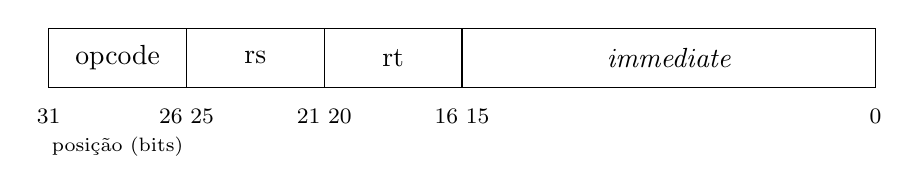
\begin{tikzpicture}
    \foreach \x/\field/\pos in {0/opcode/31,1/rs/{26 25},2/rt/{21
        20}} {
      \draw (\x*\mywidth,0) rectangle (\x*\mywidth+\mywidth,\myheight);
      \node at (\x*\mywidth+\mywidth/2, \myheight/2) {\field};
      \node at (\x*\mywidth, -\myheight/2) {\footnotesize\pos};
    }
    \draw (3*\mywidth,0) rectangle (6*\mywidth,\myheight);
    \node at (4*\mywidth+\mywidth/2, \myheight/2) {\em immediate};
    \node at (3*\mywidth, -\myheight/2) {\footnotesize 16 15};

    \node at (6*\mywidth, -\myheight/2) {\footnotesize 0};
    \node at (\mywidth/2, -\myheight) {\scriptsize posição (bits)};
\end{tikzpicture}
\smallskip
\hrule
\bigskip
Exemplo:\\

\begin{tt}
  \hspace{2cm} lw \$t0, 32(\$t1)\\
\end{tt}
{\small\color{gray} \# lw -- opcode, rs $\leftarrow$ \$t1, rt
  $\leftarrow$ \$t0, {\em immediate} $\leftarrow$ 32}\\
\bigskip
  \begin{tikzpicture}
    \foreach \x/\field/\nbits/\ndec in
    {0/\only<1>{100011}/op - 6/\only<2>{\dec{35}},1/\only<1>{10010}/\$t1 -
      5/\only<2>{\dec{9}},2/\only<1>{01000}/\$t0 - 5/\only<2>{\dec{8}}} {
      \draw (\x*\mywidth,0) rectangle (\x*\mywidth+\mywidth,\myheight);
      \node at (\x*\mywidth+\mywidth/2, \myheight/2) {\field\ndec};
      \node at (\x*\mywidth+\mywidth/2, -\myheight/2) {\footnotesize\nbits{} bits};
    }
    \draw (3*\mywidth,0) rectangle (6*\mywidth,\myheight);
    \node at (4*\mywidth+\mywidth/2, \myheight/2) {\only<1>{0000
        0000 0010 0000}\only<2>{\dec{32}}};
    \node at (4*\mywidth+\mywidth/2, -\myheight/2) {\footnotesize 16 bits};
\end{tikzpicture}

\end{block}  

\end{frame}


\begin{frame}{Formato básico das instruções MIPS}{Formato J}

  \def\mywidth{1.75cm}
  \def\myheight{0.75cm}

\begin{block}{Formato J ({\em jump})}
  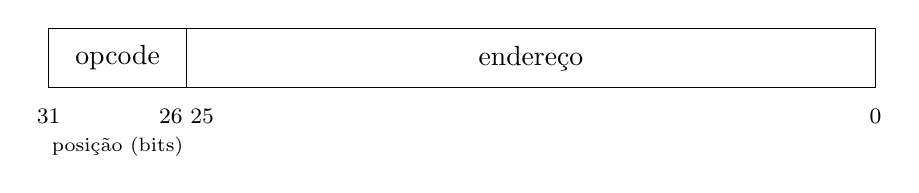
\begin{tikzpicture}
    \draw (0,0) rectangle (\mywidth,\myheight);
    \node at (\mywidth/2, \myheight/2) {opcode};
    \node at (0, -\myheight/2) {\footnotesize 31};
    
    \draw (\mywidth,0) rectangle (6*\mywidth,\myheight);
    \node at (3*\mywidth+\mywidth/2, \myheight/2) {endereço};
    \node at (\mywidth, -\myheight/2) {\footnotesize 26 25};

    \node at (6*\mywidth, -\myheight/2) {\footnotesize 0};
    \node at (\mywidth/2, -\myheight) {\scriptsize posição (bits)};
\end{tikzpicture}
\smallskip
\hrule
\bigskip
Exemplo:\\

\begin{tt}
  \hspace{2cm} j Exit\\
\end{tt}
{\small\color{gray} \# j -- opcode, Exit -- rótulo (endereço)}\\
\bigskip
  \begin{tikzpicture}
    \draw (0,0) rectangle (\mywidth,\myheight);
    \node at (\mywidth/2, \myheight/2) {\only<1>{000010}\only<2>{\dec{2}}};
    \node at (\mywidth/2, -\myheight/2) {\footnotesize op - 6 bits};
      
      \draw (\mywidth,0) rectangle (6*\mywidth,\myheight);
      \node at (3*\mywidth+\mywidth/2, \myheight/2) {\only<1>{00 0000 0000 0000
          0100 1011 0000}\only<2>{\dec{1200}}};
      \node at (3*\mywidth+\mywidth/2, -\myheight/2) {\footnotesize 26 bits};
\end{tikzpicture}

\end{block}  

\end{frame}






\def\bit#1{{\tt #1}}
\def\comment#1{{\tiny #1}}
\def\linelabel#1{{\tiny #1}}

\def\reg{\only<2>{\color{red}}\only<3->{\color{gray}}}
\def\immed{\only<3>{\color{red}}\only<2,4->{\color{gray}}}
\def\jump{\only<4>{\color{red}}\only<2,3,5->{\color{gray}}}

\begin{frame}
  \frametitle{Instru\c{c}\~oes MIPS} 

% pg 128
  
\begin{scriptsize}
\begin{tabular}[ht]{|l|c|c|c|c|c|c|l|}\hline
  \multicolumn{1}{|c|}{Nome} & \multicolumn{6}{|c|}{Campos} & \multicolumn{1}{|c|}{Descri\c{c}\~ao} \\ \hline
  
  \linelabel{Tamanho} &\bit{6} & \bit{5} & \bit{5} & \bit{5} & \bit{5} & \bit{6} &
  \comment{Todas as intru\c{c}\~oes MIPS s\~ao de 32 bits} \\ \hline
  
  \reg \linelabel{Formato-\bf{R}} & \reg op & \reg rs & \reg rt & \reg
  rd & \reg \tt{shamt} & \reg funct & \reg
  \comment{Formato de instru\c{c}\~ao aritm\'etica} \\ \hline

  \immed \linelabel{Formato-\bf{I}} & \immed op & \immed rs & \immed
  rt &  \multicolumn{3}{|c|}{\immed endere\c{c}o/imediato} &
  \immed \comment{Formato de transferência, desvio e constante} \\ \hline
  
  \jump \linelabel{Formato-\bf{J}} & \jump op & \multicolumn{5}{|c|}{\jump endere\c{c}o} &
  \jump \comment{Formato de instru\c{c}\~{a}o {\em jump}} \\ \hline
\end{tabular}


\only<1>{
\vspace{0.64cm}
% pg 100
\begin{tabular}[ht]{|l|c|c|c|c|c|c|c|l|}\hline

  \multicolumn{1}{|c|}{Nome} & Formato & \multicolumn{6}{|c|}{Exemplo} & \multicolumn{1}{|c|}{Descri\c{c}\~ao} \\ \hline
  
  add & R & 0 & 18 & 19 & 17 & 0 & 32 & add \tt{\$s1,\$s2,\$s3} \\
  \hline

  sub & R & 0 & 18 & 19 & 17 & 0 & 34 & sub \tt{\$s1,\$s2,\$s3} \\
  \hline

    addi & I & 35 & 18 & 17 & \multicolumn{3}{|c|}{100} &  addi
    \tt{\$s1,\$s2,100} \\ \hline
    
    lw & I & 43 & 18 & 17 & \multicolumn{3}{|c|}{100} &  lw
    \tt{\$s1,\$s2,100(\$s2)} \\ \hline

    sw & I & 8 & 18 & 17 & \multicolumn{3}{|c|}{100} &  sw
    \tt{\$s1,\$s2,100(\$s2)} \\ \hline

   % jr & I & 31 & \multicolumn{5}{|c|}{31} &  jr \tt{\$ra} \\ \hline

\end{tabular}
} % only 1

\only<2->{
\begin{block}{\alert<2>{Instru\c{c}\~oes reg-reg (op == 0)}}
  \only<2>{
  \begin{tabular}[ht]{ll}
      -- add, sub, and, or, nor, xor, slt & \texttt{R[rd] $\leftarrow$
        R[rs] funct R[rt]; \hfill PC $\leftarrow$ PC + 4;} \\
      -- sll, srl, sra & \texttt{R[rd] $\leftarrow$ R[rt] shift shamt;} \\
    \end{tabular}
  }
\end{block}
}

\only<3->{
\begin{block}{\alert<3>{Instru\c{c}\~oes reg-const (op != 0)}}
  \only<3>{
  \begin{tabular}[ht]{ll}
    -- addi, andi, ori, xori  & \texttt{R[rd] $\leftarrow$
      R[rs] op lm 16}; \\
      -- lui, addiu, slti, sltiu & \\
      -- lw, lh, lhu, lb, lbu & \texttt{R[rt] $\leftarrow$ Mem[ R[rs]
        + signEx(lm 16) ];} \\
      -- sw, sh, sb & \texttt{Mem[R[rs] + signEx(lm 16)]
        $\leftarrow$ R[rt];} \\
    \end{tabular}
  }
\end{block}
}


\only<4->{
\begin{block}{\alert<4>{\em Jumps}}
  \only<4>{
  \begin{tabular}[ht]{ll}
    -- j  & \texttt{PC $\leftarrow$ PC$_{31,28}$ || endere\c{c}o || 00;} \\
      -- jal & \texttt{PC $\leftarrow$ PC$_{31,28}$ || endere\c{c}o ||
        00; \hfill R[31] $\leftarrow$ PC + 4;} \\
      -- jr & \texttt{PC $\leftarrow$ R[rs];} \\
    \end{tabular}
  }
\end{block}
}

\only<5->{
\begin{block}{\alert<4>{Desvios}}
  \only<5>{
  \begin{tabular}[ht]{ll}
    -- beq, ben  & \texttt{PC $\leftarrow$ (R[rs] ?= R[rt]) ? PC +
      signEx(lm 16) : PC + 4;} \\
      -- blt, bgt, ble, bgte & \texttt{pseudo instru\c{c}\~oes} \\
    \end{tabular}
  }
\end{block}
}



\end{scriptsize}


\end{frame}





\begin{frame}{TODO}
  
  \begin{itemize}
  \item loops
  \item MARS
  \item tabela mips
  \end{itemize}

\end{frame}

%%% Local Variables:
%%% TeX-master: main
%%% End:

